\section{Theorie}
\label{sec:Theorie}
Ein ungedämpfter Schwingkreis besteht aus zwei Energiespeichern: eine Kapazität C
in Form eines Kondensators und eine Induktivität L in Form einer Spule. Befindet
sich Energie in dem System, so fliesst der Strom periodisch wechselnd von der
Kapazität zur Induktivität und umgekehrt. In einem idealen System bleibt die Energie
dabei erhalten.
Fügt man diesem Schwingkreis einen ohmschen Widerstand R hinzu, so erhält man eine
gedämpfte Schwingung, da an dem Widerstand kontinuierlich Energie als Joulsche Wärme
abfällt. Infolgedessen nehmen die Amplitude des Stroms und die Spannung am
Kondensator mit der Zeit ab. Ein solcher gedämpfter Schwingkreis ist in Abbildung
\ref{fig:gedaempfter_schwingkreis} zu sehen.
\begin{figure}
  \centering
  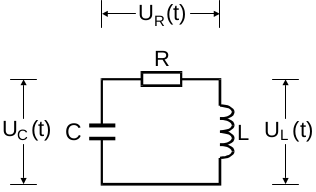
\includegraphics[width=0.4\textwidth]{gedaempfter_schwingkreis.png}
  \caption{Gedämpfter Schwingkreis mit einer Kapazität C, einem ohmschen Widerstand R
  und einer Induktivität L in einer Reihenschaltung.}
  \label{fig:gedaempfter_schwingkreis}
\end{figure}
Wird an den Schwingkreis eine periodische Spannung angelegt, führt dies zu einer
erzwungenen Schwinung. Das System schwingt dann mit der Frequenz der angelegten
Spannung und nicht mehr mit seiner Eigenfrequenz.
\cite{sample}
